\chapter{Canais de Comunicação}

Na essência da teoria da informação, um dos problemas centrais é 
reproduzir, em um ponto, uma mensagem selecionada em outro ponto, seja de
maneira exata ou aproximada. Os \emph{canais de comunicação}\index{canal}\index{canal de comunicação|see{canal}} modelam a transmissão de
informação através de um meio físico ou lógico, frequentemente sujeito a
imperfeições. O estudo dos canais busca responder a duas questões fundamentais: como
garantir a confiabilidade da transmissão? e qual é a taxa máxima de comunicação
possível em um dado sistema? Antes do trabalho seminal de Claude Shannon,
acreditava-se que, para alcançar uma probabilidade de erro nula, seria
necessário reduzir a taxa de transmissão a zero. Shannon, no entanto, mostrou
que é possível transmitir informações com uma probabilidade de erro que tende a
zero, desde que a taxa de comunicação não exceda um limite fundamental: a
\emph{capacidade do canal}\index{canal!capacidade}.

Canais de comunicação estão presentes em uma ampla variedade de contextos
práticos. Exemplos incluem a transmissão de sinais via rádio, satélite ou redes
celulares (tranmissão entre dois pontos no espaço); a leitura e escrita em
discos rígidos ou memórias eletrônicas, onde bits são gravados e recuperados de
superfícies físicas (transmissão entre dois instantes de tempo); e até mesmo
sistemas biológicos, como a comunicação entre neurônios. Em todos esses casos,
o canal é o meio que conecta a fonte ao receptor, e seu desempenho é limitado
por fatores como ruído, interferência ou degradação do sinal.

Um modelo típico de canal de comunicação considera a presença de ruído, uma
perturbação aleatória que corrompe a mensagem transmitida. As fontes de ruído
podem ser diversas: térmicas, como o movimento aleatório de elétrons em
circuitos; externas, como interferência de outros sinais; ou intrínsecas ao
meio, como dispersão em fibras ópticas. Para estudar esses fenômenos,
recorremos a modelos simplificados de canais. Esses modelos, embora
idealizados, capturam características essenciais dos sistemas reais, e nos
permitem tratar matemáticamente o problema e compreender o problema.

Uma questão fundamental é a separação entre o codificador de fonte e o
codificador de canal, um conceito proposto por Claude Shannon. O codificador de
fonte comprime os dados de entrada, removendo redundâncias para uma
representação eficiente da mensagem, enquanto o codificador de canal introduz
redundância controlada para proteger contra erros do canal de comunicação.
Shannon demonstrou que esses dois processos podem ser projetados de forma
independente sem comprometer a otimalidade, desde que a taxa de compressão da
fonte não ultrapasse a capacidade do canal. Essa abordagem simplifica o projeto
de sistemas de comunicação.


\subsection{Código de Repetição: Uma Introdução à Codificação de Canal}

A \emph{codificação de canal}\index{canal!codificação} é uma técnica essencial para garantir a confiabilidade
da transmissão de informação através de canais ruidosos, e um dos exemplos mais
simples é o código de repetição. Nesse esquema, cada bit da mensagem é
repetido um número fix mesmo de vezes, formando um código de comprimento maior.
Por exemplo, no código de repetição tripla, o bit $0$ é codificado como $000$ e
o bit $1$ como $111$. No receptor, a decisão é tomada por votação majoritária:
se a sequência recebida for $010$, o bit decodificado será $0$, pois há mais
zeros do que uns. Esse método é intuitivo e serve como uma introdução
pedagógica aos conceitos de redundância e correção de erros.

O código de repetição é um código muito simples e intuitivo.
Ainda assim, ele pode reduzir a probabilidade de erro em canais ruidosos. 
Por exemplo, em um canal binário simétrico com probabilidade de erro $p$, repetir um bit
três vezes diminui a chance de erro de $p$ para $p^2(1-p) + p^3$, que é menor
que $p$ para qualquer valor de $p$. Isso ocorre porque o erro só persiste
se pelo menos dois dos três bits forem corrompidos, um evento menos provável.

No entanto, o código de repetição também possui desvantagens significativas. A
mais evidente é a redução drástica da taxa de transmissão: ao repetir cada bit
$n$ vezes, a taxa cai para $1/n$ da taxa original, tornando-o ineficiente.
Além disso, sua capacidade de correção é limitada;
ele só corrige erros se menos da metade dos bits repetidos forem afetados, o
que o torna menos robusto em canais com altas taxas de erro.





\subsection{Definições Fundamentais sobre Canais de Comunicação}

Para compreender o estudo dos canais de comunicação, é
essencial estabelecer definições de alguns conceitos fundamentais que
descrevem seu comportamento e desempenho.

\begin{definition}[Canal Discreto]
  Um \emph{canal discreto}\index{canal!discreto} é caracterizado por um conjunto finito ou contável de símbolos de entrada $X$,
  um conjunto finito ou contável de símbolos de saída $Y$, e uma relação probabilística entre eles, definida por
  uma matriz de transição condicional $p(y|x)$. Essa matriz especifica a
  probabilidade de receber o símbolo $y \in Y$ dado que o símbolo $x \in X$ foi transmitido.
\end{definition}

\begin{definition}[Canal sem memória]
  Um canal é dito \emph{sem memória}\index{canal!sem memória} se a saída em um dado instante $t$ depende apenas do
símbolo de entrada correspondente naquele instante $t$, e não de entradas ou saídas
anteriores, isto é, $y_t \independent x_{1:t-1} \mid x_t$.
Formalmente, para um canal discreto, a probabilidade condicional da
sequência de saídas $y_1, y_2, \dots, y_n$ dado um conjunto de entradas 
$x_1, x_2, \dots, x_n$ é dada por 
$p(y_1, y_2, \dots, y_n | x_1, x_2, \dots, x_n) = \prod_{i=1}^n p(y_i | x_i)$. 
Essa propriedade simplifica a análise, pois
elimina dependências temporais.
\end{definition}

\begin{definition}[Taxa de Fluxo de Informação]
A \emph{taxa de fluxo de informação}\index{canal!taxa de fluxo de informação} através de um canal mede a quantidade de
informação que pode ser transmitida de forma confiável através do canal por
uso. Para um canal discreto com entrada $X$ e saída $Y$, ela é dada pela
informação mútua $I(X;Y)$, depende assim da distribuição de probabilidade das
entradas $p(x)$ e das características do canal $p(y|x)$.
\end{definition}

\begin{definition}[Taxa]
  A \emph{taxa}\index{canal!taxa}\index{código!taxa} de um sistema de comunicação é definida como a quantidade média de
informação transmitida por uso do canal, geralmente expressa em bits por
utilização do canal. Para um código com $M$ mensagens possíveis transmitidas em
$n$ usos do canal, a taxa é dada por $R = \sfrac{\log_2 M}{n}$.
\end{definition}

\begin{definition}[Capacidade de Canal]
  A \emph{capacidade de um canal}\index{canal!capacidade} é o limite superior da taxa na qual a informação pode
ser transmitida com uma probabilidade de erro que tende a zero à medida que o
comprimento do código aumenta. Para um canal discreto sem
memória, a capacidade $C$ é definida como
\begin{equation}
  C \triangleq \max_{p(x) \in \Delta} I(X;Y)
\end{equation}
onde a
maximização é feita sobre todas as distribuições de probabilidade possíveis
para a entrada $X$.
\end{definition}






\section{Modelos de Canais}

\subsection{Canal binário sem ruído}

\begin{marginfigure}%
  \centering
  \begin{tikzpicture}[node distance=1cm, >=Stealth]
    \node (x0) at (0, 0) {0};
    \node (x1) [below=1cm of x0] {1}; % Ensure consistent vertical spacing

    \node (X_label) at ($(x0.north)!0.5!(x1.south)$) [left=0.5cm of x0, yshift=-0.75cm] {$X$};

    \node (y0) at (2, 0) {0}; % Aligned horizontally with x0
    \node (y1) [below=1cm of y0] {1}; % Aligned horizontally with x1

    \node (Y_label) at ($(y0.north)!0.5!(y1.south)$) [right=0.5cm of y0, yshift=-0.75cm] {$Y$};

    \draw [->] (x0) -- (y0);
    \draw [->] (x1) -- (y1);

    \node [below=0.5cm of x1, xshift=-1cm] {$\mathcal{X} = \{0,1\}$};
    \node [below=0.5cm of y1, xshift=1cm] {$\mathcal{Y} = \{0,1\}$}; % Changed xshift to -1cm for consistency
  \end{tikzpicture}
  %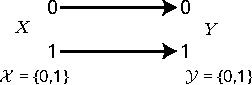
\includegraphics[width=\linewidth]{figures/bsc.pdf}
  \caption{Representação esquemática de um canal binário sem ruído.}\label{fig:bsc}
\end{marginfigure}

O \emph{canal binário sem ruído}\index{canal!binário sem ruído} é o modelo mais simples de canal discreto, onde o
alfabeto de entrada e saída é binário, $\mathcal{X} = \mathcal{Y} = \{0, 1\}$,
e a transmissão ocorre sem erros. A forma esquemática de representação deste canal
é apresentada na \Cref{fig:bsc}. A matriz de transição é dada por $p(y|x) = 1$
se $y = x$ e $p(y|x) = 0$ se $y \neq x$. Nesse caso, a saída é uma cópia exata da entrada, e
a capacidade do canal é $C = 1$ bit por uso, pois a informação mútua $I(X;Y) = H(X)$ 
atinge seu máximo quando os símbolos são equiprováveis. Este modelo
representa um sistema ideal, útil como referência para comparar canais ruidosos.



\subsection{Canal com ruído e saídas sem sobreposição}

\begin{marginfigure}%
  \centering
  \begin{tikzpicture}[
    node distance=1cm,          % Default distance between nodes
    >=Stealth,                  % Default arrow tip style
    arrowlabel/.style={font=\small, inner sep=1pt} % Style for labels on arrows
]

    % --- Input set X and its elements ---
    % Define element nodes for X
    \node (x0) at (0, 0.5) {0}; % Adjusted y-coordinate to provide space for branching
    \node (x1) [below=1.5cm of x0] {1}; % Increased vertical spacing between 0 and 1

    % Place X label vertically centered between x0 and x1
    \node (X_label) at ($(x0.north)!0.5!(x1.south)$) [left=0.5cm of x0, yshift=-1.1cm] {$X$};

    % --- Output set Y and its elements ---
    % Define element nodes for Y
    \node (y_a) at (3, 1.25) {a}; % Position 'a'
    \node (y_b) [below=0.75cm of y_a] {b}; % Position 'b' below 'a'
    \node (y_c) [below=0.75cm of y_b] {c}; % Position 'c' below 'b' (larger gap)
    \node (y_d) [below=0.75cm of y_c] {d}; % Position 'd' below 'c'

    % Place Y label vertically centered between y_a and y_d (topmost and bottommost Y elements)
    \node (Y_label) at ($(y_a.north)!0.5!(y_d.south)$) [right=0.5cm of y_d, yshift=1.75cm] {$Y$};

    % --- Arrows with labels ---
    % From 0 to a
    \draw [->] (x0) -- (y_a) node[midway, above, arrowlabel] {$\sfrac{1}{2}$};
    % From 0 to b
    \draw [->] (x0) -- (y_b) node[midway, below, arrowlabel] {$\sfrac{1}{2}$};
    % From 1 to c
    \draw [->] (x1) -- (y_c) node[midway, above, arrowlabel] {$\sfrac{1}{2}$};
    % From 1 to d
    \draw [->] (x1) -- (y_d) node[midway, below, arrowlabel] {$\sfrac{1}{2}$};

    % --- Set definitions ---
    \node [below=1cm of x1, xshift=-0.75cm] {$\mathcal{X} = \{0,1\}$}; % Adjusted position and anchor
    \node [below=1cm of x1, xshift=4cm] {$\mathcal{Y} = \{a,b,c,d\}$}; % Adjusted position and anchor

  \end{tikzpicture}
  %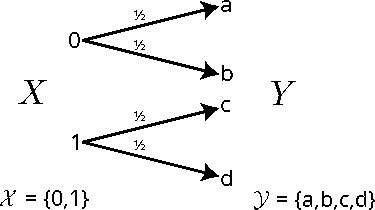
\includegraphics[width=\linewidth]{figures/nonc.pdf}
  \caption{Canal com ruído sem sobreposição na saída.}\label{fig:nonc}
\end{marginfigure}

Um \emph{canal com ruído e saídas sem sobreposição}\index{canal!com ruído e sem sobreposição} é caracterizado por um alfabeto de
entrada $\mathcal{X}$ e um alfabeto de saída $\mathcal{Y}$, onde cada símbolo de entrada $x \in \mathcal{X}$
produz uma saída $y \in \mathcal{Y}$ pertencente a um subconjunto disjunto $S_x \subseteq \mathcal{Y}$,
com probabilidade condicional $p(y|x) > 0$ apenas para $y \in S_x$. Por
exemplo, considere um canal com $\mathcal{X} = \{0, 1\}$ e $\mathcal{Y} = \{a, b, c, d\}$, 
onde $0$ pode gerar saídas $\{a, b\}$ e $1$ pode gerar $\{c, d\}$, com $S_0 = \{a, b\}$ e $S_1 = \{c, d\}$
disjuntos. Este canal exemplo é apresentado na \Cref{fig:nonc}.
O ruído está presente na escolha aleatória dentro de $S_x$, mas a
ausência de sobreposição entre os subconjuntos permite identificar a entrada
com base na saída. Esse modelo é útil para estudar sistemas onde o ruído não
causa confusão entre símbolos distintos.




\subsection{Canal de permutação}

\begin{marginfigure}%
  \centering
  %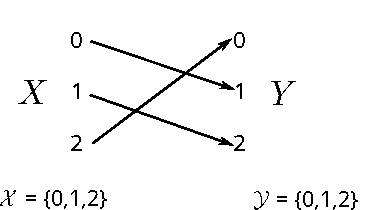
\includegraphics[width=\linewidth]{figures/canalperm.pdf}
  \begin{tikzpicture}[
    node distance=1cm, % Default distance between nodes
    >=Stealth,         % Default arrow tip style (modern arrow)
    element/.style={inner sep=1pt} % Style for the numbers 0, 1, 2
]

    % --- Input set X and its elements ---
    % Define element nodes for X
    \node[element] (x0) at (0, 1) {0};
    \node[element] (x1) [below=0.75cm of x0] {1}; % Slightly reduced spacing to fit 3 elements
    \node[element] (x2) [below=0.75cm of x1] {2};

    % Place X label vertically centered between x0 and x2
    \node (X_label) at ($(x0.north)!0.5!(x2.south)$) [left=0.5cm of x1] {$X$};

    % --- Output set Y and its elements ---
    % Define element nodes for Y, horizontally aligned with X elements
    \node[element] (y0) at (2.5, 1) {0}; % Adjusted x-coordinate for overall diagram width
    \node[element] (y1) [below=0.75cm of y0] {1};
    \node[element] (y2) [below=0.75cm of y1] {2};

    % Place Y label vertically centered between y0 and y2
    \node (Y_label) at ($(y0.north)!0.5!(y2.south)$) [right=0.5cm of y1] {$Y$};

    % --- Arrows representing the permutation ---
    \draw [->] (x0) -- (y1); % 0 -> 1
    \draw [->] (x1) -- (y2); % 1 -> 2 
    \draw [->] (x2) -- (y0); % 2 -> 0 

    % --- Set definitions ---
    \node [below=0.75cm of x2, xshift=-1.5cm, anchor=north west] {$\mathcal{X} = \{0,1,2\}$};
    \node [below=0.75cm of y2, xshift=1.5cm, anchor=north east] {$\mathcal{Y} = \{0,1,2\}$};

  \end{tikzpicture}
  \caption{Exemplo de canal de permutação.}\label{fig:canalperm}
\end{marginfigure}

O \emph{canal de permutação}\label{canal!de permutação} é um modelo determinístico onde o alfabeto de entrada e
saída é o mesmo, $\mathcal{X} = \mathcal{Y}$, e cada entrada $x$ é mapeada para uma saída 
$y = \pi(x)$, onde $\pi$ é uma permutação fixa dos símbolos de $\mathcal{X}$. Por exemplo, se
$\mathcal{X} = \{0, 1, 2\}$ e $\pi(0) = 1$, $\pi(1) = 2$, $\pi(2) = 0$, a saída é uma
reorganização previsível da entrada. A \Cref{fig:canalperm} apresentada o esquemático
do canal de permutação proposto neste exemplo.
Como a permutação é biunívoca, não há
perda de informação, e a capacidade do canal é $C = \log |\mathcal{X}|$ bits por uso, uma vez que
\begin{subequations}
  \begin{align}
    C &= \max_{p(x)} I(X;Y) \\
      &= \max_{p(x)} H(X) - \underbrace{H(X|Y)}_{=0} \\
      &= \max_{p(x)} H(X) \\
      &= \log |\mathcal{X}| ,
  \end{align}
\end{subequations}
sendo assim, a distribuição uniforme na entrada é aquela que maximiza a informação
mútua e alcança assim a capacidade do canal. 




\subsection{Canal binário simétrico}

\begin{marginfigure}%
  \centering
  %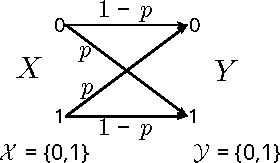
\includegraphics[width=\linewidth]{figures/bsch.pdf}
  \begin{tikzpicture}[
    node distance=1.5cm,
    >=Stealth,
    prob/.style={font=\footnotesize, inner sep=1pt}
]

    % Input set X
    \node (X_label) at (-1, -0.5) {$X$};
    \node (x0) at (0, 0.5) {0};
    \node (x1) [below=of x0] {1};

    % Output set Y
    \node (Y_label) at (4, -0.5) {$Y$};
    \node (y0) at (3, 0.5) {0};
    \node (y1) [below=of y0] {1};

    % Arrows
    \draw [->] (x0) -- (y0) node [above, midway, prob] {$1 - p$};
    \draw [->] (x0) -- (y1) node [below, midway, prob, xshift=-1cm, yshift=-0.15cm] {$p$};
    \draw [->] (x1) -- (y0) node [above, midway, prob, xshift=-1cm, yshift=0.15cm] {$p$};
    \draw [->] (x1) -- (y1) node [below, midway, prob] {$1 - p$};

    % Set definitions
    \node [below=0.75cm of x1, align=center] {$\mathcal{X} = \{0,1\}$};
    \node [below=0.75cm of y1, align=center] {$\mathcal{Y} = \{0,1\}$};

  \end{tikzpicture}
  \caption{Canal binário simétrico.}\label{fig:bsch}
\end{marginfigure}

O \emph{canal binário simétrico} (CBS)\index{canal!binário simétrico} é um dos modelos mais estudados, com alfabeto
de entrada e saída $\mathcal{X} = \mathcal{Y} = \{0, 1\}$ e uma probabilidade de erro $p$, onde
$p(y=1|x=0) = p(y=0|x=1) = p$ e $p(y=x|x) = 1-p$, para $0 \leq p \leq 1/2$. 
Este canal é representado na \Cref{fig:bsch}. 
A simetria implica que o erro é igualmente provável em ambas as direções. A
capacidade do CBS é dada por 
\begin{subequations}\label{eq:capbsch}
  \begin{align}
    C &= \max_{p(x)} I(X;Y) \\
      &= \max_{p(x)} H(Y) - H(Y|X) \\
      &= \max_{p(x)} H(Y) - \sum_x p(x) H(Y|X=x) \\
      &= \max_{p(x)} H(Y) - \sum_x p(x) H(p) \\
      &= \max_{p(x)} H(Y) - h(p) \\
      &= 1 - h(p) , \label{dem:capbschA}
  \end{align}
\end{subequations}
onde $H(p) = h(p) = -p \log p - (1-p) \log (1-p)$ é a entropia binária,
e utilizamos em \ref{dem:capbschA} a simetria do problema, que
nos garante que a distribuição uniforme na entrada acarreta
a distribuição uniforme na saída, maximizando $H(Y)$. Logo,
a distribuição na entrada que alcança a capacidade de canal
é a distribuição uniforme.


\subsection{Canal binário com apagamento}

\begin{marginfigure}%
  \centering
  %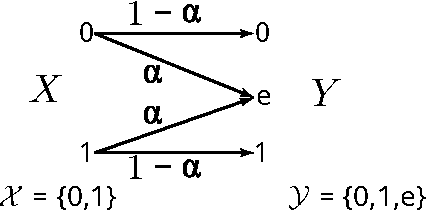
\includegraphics[width=\linewidth]{figures/bech.pdf}
  \begin{tikzpicture}[
    node distance=1.5cm,
    >=Stealth,
    prob/.style={font=\footnotesize, inner sep=1pt}
]

    % Input set X
    \node (X_label) at (-1, -0.5) {$X$};
    \node (x0) at (0, 0.5) {0};
    \node (x1) [below=of x0] {1};

    % Output set Y
    \node (Y_label) at (4, -0.5) {$Y$};
    \node (y0) at (3, 0.5) {0};
    \node (ye) at (3, -0.5) {e};
    \node (y1) at (3, -1.5) {1};

    % Arrows
    \draw [->] (x0) -- (y0) node [above, midway, prob] {$1 - \alpha$};
    \draw [->] (x0) -- (ye) node [below left=2pt, midway, prob] {$\alpha$};
    \draw [->] (x1) -- (ye) node [above left=2pt, midway, prob] {$\alpha$};
    \draw [->] (x1) -- (y1) node [below, midway, prob] {$1 - \alpha$};

    % Set definitions
    \node [below=0.75cm of x1, align=center] {$\mathcal{X} = \{0,1\}$};
    \node [below=0.75cm of y1, align=center] {$\mathcal{Y} = \{0,1,e\}$};

  \end{tikzpicture}
  \caption{Canal binário com apagamento.}\label{fig:bech}
\end{marginfigure}

O \emph{canal binário com apagamento} (CBA)\index{canal!binário com apagamento} possui um alfabeto de entrada 
$\mathcal{X} = \{0, 1\}$ e um alfabeto de saída $\mathcal{Y} = \{0, 1, e\}$, 
onde $e$ representa um apagamento. Nesse modelo, cada símbolo de entrada é transmitido corretamente
com probabilidade $1-\alpha$, ou seja, $p(y=x|x) = 1-\alpha$, ou é apagado com
probabilidade $\alpha$, ou seja, $p(y=e|x) = \alpha$, para $0 \leq \alpha \leq 1$. 
Não há erro de inversão ($p(y=1|x=0) = p(y=0|x=1) = 0$).
Este canal é ilustrado na \Cref{fig:bech}.
Para obter a capacidade deste canal, prosseguimos da seguinte forma:
\begin{subequations}\label{eq:capcanalapagamento}
  \begin{align}
    C &= \max_{p(x)} I(X;Y) \\ 
      &= \max_{p(x)} \left(H(Y) - H(Y|X)\right) \\
      &= \max_{p(x)} \left(H(Y) - H(\alpha)\right) \\
      &= \max_{p(x)} \left(H(E) + H(Y|E) - H(\alpha)\right) \label{eq:demcapcanalapagA}\\
      &= \max_{p(x)} \left(H(\alpha) + (1 - \alpha) H(\pi) - H(\alpha)\right) \label{eq:demcapcanalapagB}\\ 
      &= \max_{p(x)} (1 - \alpha) H(\pi) \label{eq:demcapcanalapagC} \\
      &= 1 - \alpha ,
  \end{align}
\end{subequations}
onde em \ref{eq:demcapcanalapagA} utilizamos a regra da cadeia:
\begin{subequations}
  \begin{align}
    H(Y,E) &= H(E) + H(Y|E) \\
           &= H(Y) + \bcancelto{0}{H(E|Y)} ,
  \end{align}
\end{subequations}
e em \ref{eq:demcapcanalapagB} utilizamos
\begin{subequations}
  \begin{align}
    H(Y|E) &= \alpha H(Y|Y=e) + (1-\alpha) H(Y|Y\neq e) \\
           &= \alpha \cdot 0 + (1-\alpha) H(\pi) .
  \end{align}
\end{subequations}
Note que também podemos obter a equivalência entre a escolha sob $Y$ 
e a quebra desta escolha em duas: houve ou não apagamento; e caso não tenha
ocorrido apagamento, qual valor observado, 0 ou 1, com probabilidade $\pi$ e
$1-\pi$. Esta equivalência é ilustrada na \Cref{fig:eqvh} e a relação entre as
incertezas é expressa a seguir:
\begin{subequations}
  \begin{align}
    H(Y) &= H\left( \overbrace{(1-\pi)(1-\alpha)}^{\text{se }Y=0} , \overbrace{\alpha}^{\text{se }Y=e} , \overbrace{\pi(1-\alpha)}^{\text{se }Y=1} \right) \\
         &= H(\alpha) + (1 - \alpha) H(\pi) .
  \end{align}
\end{subequations}
\begin{marginfigure}%
  \centering
  \begin{tikzpicture}[
    line width=1pt, % Make lines a bit thicker
    font=\small      % Set default font size for labels
]

    % --- Left Tree ---
    \coordinate (L_center) at (0,0); % Center point for the left tree

    % Branches from L_center
    \draw (L_center) -- ($(L_center) + (1, 1)$) node[midway, sloped, above] {$(1-\pi)(1-\alpha)$};
    \draw (L_center) -- ($(L_center) + (1, 0)$) node[midway, sloped, above] {$\alpha$};
    \draw (L_center) -- ($(L_center) + (1, -1)$) node[midway, sloped, below] {$\pi(1-\alpha)$};

    % --- Equivalence Symbol ---
    \node at (1.5, 0) {$\equiv$};

    % --- Right Tree ---
    \coordinate (R_center) at (2,0); % Center point for the right tree

    % Main branch from R_center
    \draw (R_center) -- ($(R_center) + (2, 1)$) node[midway, sloped, above] {$\alpha$};

    % Sub-branching point
    \coordinate (R_branch_point) at ($(R_center) + (1, -1)$);
    \draw (R_center) -- (R_branch_point) node[midway, sloped, below] {$(1-\alpha)$}; % First segment label

    % Sub-branches from R_branch_point
    \draw (R_branch_point) -- ($(R_branch_point) + (1, 0.5)$) node[midway, sloped, above] {$(1-\pi)$};
    \draw (R_branch_point) -- ($(R_branch_point) + (1, -0.5)$) node[midway, sloped, below] {$\pi$};

  \end{tikzpicture}
  %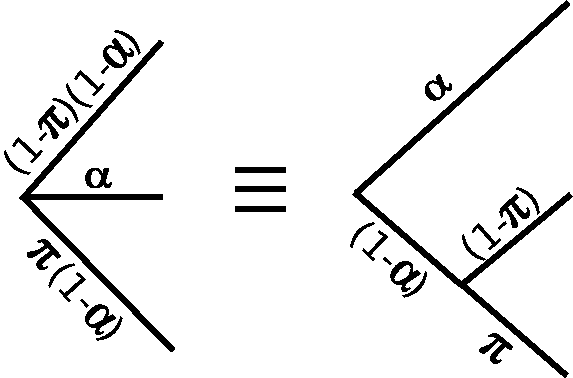
\includegraphics[width=\linewidth]{figures/eqvh.pdf}
  \caption{Incertezas equivalentes.}\label{fig:eqvh}
\end{marginfigure}
A capacidade do canal é $C = 1-\alpha$ bits por uso, 
pois apenas a fração $1-\alpha$ das transmissões contribui para a
informação recebida. Este modelo é relevante para sistemas como redes de
pacotes, onde dados podem ser perdidos, mas não corrompidos.






\subsection{Canal de confusão ternário}

\begin{marginfigure}%
  \centering
  %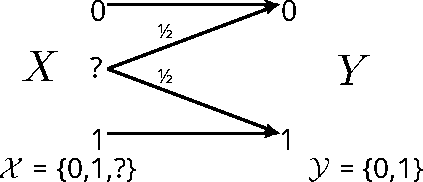
\includegraphics[width=\linewidth]{figures/tcc.pdf}
  \begin{tikzpicture}[
    node distance=1.5cm, % Default distance between nodes
    >=Stealth,           % Default arrow tip style (modern arrow)
    prob/.style={font=\small, fill=white, inner sep=1pt} % Style for labels on arrows
]

    % --- Input set X and its elements ---
    % Define element nodes for X
    \node (x0) at (0, 1) {0};
    \node (x_q) [below=1cm of x0] {?}; % The unknown element
    \node (x1) [below=1cm of x_q] {1};

    % Place X label vertically centered between x0 and x1
    \node (X_label) at ($(x0.north)!0.5!(x1.south)$) [left=0.5cm of x_q] {$X$};

    % --- Output set Y and its elements ---
    % Define element nodes for Y, horizontally aligned
    \node (y0) at (4, 1) {0};
    \node (y1) [below=2.5cm of y0] {1}; % Adjust vertical spacing to match diagram

    % Place Y label vertically centered between y0 and y1
    \node (Y_label) at ($(y0.north)!0.5!(y1.south)$) [right=0.5cm of y0, yshift=-1.5cm] {$Y$};

    % --- Arrows ---
    \draw [->] (x0) -- (y0); % 0 -> 0 (no label)
    \draw [->] (x_q) -- (y0) node[midway, sloped, above, prob] {$\sfrac{1}{2}$}; % ? -> 0 with label
    \draw [->] (x_q) -- (y1) node[midway, sloped, below, prob] {$\sfrac{1}{2}$}; % ? -> 1 with label
    \draw [->] (x1) -- (y1); % 1 -> 1 (no label)

    % --- Set definitions ---
    \node [below=0.75cm of x1, xshift=-1cm, anchor=north west] {$\mathcal{X} = \{0,1,?\}$};
    \node [below=0.75cm of y1, xshift=1cm, anchor=north east] {$\mathcal{Y} = \{0,1\}$};

  \end{tikzpicture}
  \caption{Canal de confusão ternário.}\label{fig:tcc}
\end{marginfigure}

O \emph{canal de confusão ternário}\index{canal!confusão ternário} opera com alfabeto de entrada 
$\mathcal{X} = \{0, 1, ?\}$ e alfabeto de saída $\mathcal{Y} = \{0, 1\}$.
Neste exemplo, o símbolo $?$ representa um símbolo indeterminado na entrada.
Supondo que o símbolo indeterminado pode gerar $0$ ou $1$ na saída com igual
probabilidade, como representado na \Cref{fig:tcc}, teremos a seguinte capacidade
para este canal:
\begin{subequations}
  \begin{align}
    C &= \max_{p(x)} I(X;Y) \\
      &= \max_{p(x)} \left( H(Y) - H(Y|X) \right) \\
      &= \max_{p(x)} \left( H(Y) - \Pr(X = ?) \right) \label{dem:capcanalconfterA}\\
      &= 1 - 0 \\
      &= 1
  \end{align}
\end{subequations}
onde em \ref{dem:capcanalconfterA} utilizamos que
\begin{subequations}
  \begin{align}
    \begin{split} H(Y|X) ={}& \Pr(X=0) \underbrace{H(Y|X=0)}_{=0} + \Pr(X=?) \underbrace{H(Y|X=?)}_{=1} + \\
    & \Pr(X=1) \underbrace{H(Y|X=1)}_{=0} \end{split}\\
      ={}& \Pr(X=?) ,
  \end{align}
\end{subequations}
e o fato de que \ref{dem:capcanalconfterA} pode ser maximizado 
ao minimizar o segundo termo, requerendo $p(X=?) = 0$, e 
maximizando $H(Y)$ que pode ser obtido ao requerer $p(X=0) = p(X=1)$,
o que garante uma distribuição uniforme na saída.




\begin{definition}[Canal simétrico]
Um \emph{canal simétrico}\index{canal!simétrico} é um canal discreto cuja matriz de transição
condicional $p(y|x)$, para $x \in \mathcal{X}$ e $y \in \mathcal{Y}$, possui linhas que são
permutações umas das outras e colunas que também são permutações umas das
outras. Isso implica que a probabilidade de transição é invariante sob
re-rotulação dos símbolos de entrada e saída, simplificando a análise da
capacidade. Um canal fracamente simétrico é um canal discreto no qual
cada linha da matriz $p(y|x)$ é uma permutação de qualquer outra linha, e a
soma $\sum_{x \in \mathcal{X}} p(y|x) = p(y)$ é a mesma para todo $y \in \mathcal{Y}$, ou seja, as
saídas têm a mesma probabilidade marginal. Essas propriedades são fundamentais
para canais como o binário simétrico, onde a simetria facilita o cálculo da
capacidade máxima.
\end{definition}




\begin{theorem}[Capacidade de canais fracamente simétricos]\index{canal!capacidade!fracamente simétrico}
Para um canal discreto fracamente simétrico com alfabeto de saída $\mathcal{Y}$
e matriz de transição condicional $p(y|x)$, a capacidade $C$ é dada por
\begin{equation}
C = \log |Y| - H(r),
\end{equation}
onde $r$ representa qualquer linha da matriz $p(y|x)$, e 
$H(r) = H(Y|X=x) = -\sum_{y \in \mathcal{Y}} p(y|x) \log p(y|x)$ 
é a entropia condicional da saída
dado um símbolo de entrada $x$. Como as linhas da matriz são permutações umas
das outras, $H(Y|X=x)$ é a mesma para todo $x \in \mathcal{X}$. Essa capacidade é
atingida com uma distribuição uniforme sobre as entradas.
\end{theorem}


\begin{proof}
Seja um canal discreto fracamente simétrico com alfabeto de entrada
$\mathcal{X}$, alfabeto de saída $\mathcal{Y}$ e matriz de transição
condicional $p(y|x)$. A capacidade é definida como
\begin{equation}
C = \max_{p(x)} I(X;Y),
\end{equation}
onde $I(X;Y) = H(Y) - H(Y|X)$ é a informação mútua, e a maximização é feita
sobre todas as distribuições de probabilidade $p(x)$ das entradas.

Em um canal fracamente simétrico, cada linha da matriz $p(y|x)$ é uma
permutação de qualquer outra, o que implica que a entropia condicional
$H(Y|X=x) = -\sum_{y \in \mathcal{Y}} p(y|x) \log p(y|x)$ é a mesma para todo
$x \in \mathcal{X}$. Denote essa entropia comum por $H(r)$, onde $r$ representa
qualquer linha da matriz $p(y|x)$. Assim, a entropia condicional total é
\begin{equation}
H(Y|X) = \sum_{x \in \mathcal{X}} p(x) H(Y|X=x) = \sum_{x \in \mathcal{X}} p(x) H(r) = H(r),
\end{equation}
independente da escolha de $p(x)$.

Agora, consideremos $H(Y)$, a entropia da saída. A probabilidade marginal
$p(y)$ é dada por
\begin{equation}
p(y) = \sum_{x \in \mathcal{X}} p(x) p(y|x).
\end{equation}
Pela propriedade de simetria fraca, a soma $\sum_{x \in \mathcal{X}} p(y|x)$ é
constante para todo $y \in \mathcal{Y}$. Ou seja, a soma das probabilidades $p(y|x)$ 
na matriz de transição do canal é a mesma para todas as linhas. Seja então 
  $\alpha = \sum_{x \in \mathcal{X}} p(y|x)$ essa constante. Escolher uma distribuição uniforme para
as entradas, $p(x) = 1/|\mathcal{X}|$, nos garante uma distribuição uniforme na saída
(o que maximiza $H(Y)$). Teremos assim
\begin{equation}  
p(y) = \sum_{x \in \mathcal{X}} \frac{1}{|\mathcal{X}|} p(y|x) = \frac{1}{|\mathcal{X}|} \sum_{x \in \mathcal{X}} p(y|x) = \frac{\alpha}{|\mathcal{X}|}.
\end{equation}
Como $\alpha$ é igual para todo $y$, $p(y)$ é uniforme, isto é, $p(y) = 1/|\mathcal{Y}|$.
Assim, $H(Y) = \log |\mathcal{Y}|$.

Substituindo em $I(X;Y)$, obtemos
\begin{equation}
I(X;Y) = H(Y) - H(Y|X) = \log |\mathcal{Y}| - H(r).
\end{equation}
Assim, a informação mútua é maximizada quando $H(Y) = \log |\mathcal{Y}|$, o que ocorre com a distribuição uniforme de entrada. Portanto, a capacidade é
\begin{equation}
C = \max_{p(x)} I(X;Y) = \log |\mathcal{Y}| - H(r).
\end{equation}
\end{proof}





Os canais de comunicação frequentemente estão sujeitos a ruído, corrompendo as
mensagens transmitidas. Para garantir a confiabilidade da comunicação,
utilizamos códigos, que são esquemas para mapear mensagens em sequências
de símbolos (palavras-código) e recuperá-las no receptor, mesmo na presença de
erros. Um código é caracterizado pelo número de mensagens que pode representar
($M$) e pelo comprimento das palavras-código ($n$), com a taxa de transmissão
definida como $R = \sfrac{\log M }{n}$. A definição a seguir formaliza esses conceitos,
estabelecendo a estrutura de um código para um canal discreto.


\begin{definition}[Código $(M,n)$]
  Um \emph{código $(M,n)$}\index{código!(M,n)} para um canal discreto $(\mathcal{X}, p(y|x), \mathcal{Y})$ consiste em:
\begin{enumerate}
  \item Um conjunto de mensagens $\{1, 2, \ldots, M\}$, representando as possíveis entradas da fonte.
  \item Uma função de codificação $f: \{1, 2, \ldots, M\} \to \mathcal{X}^n$, que mapeia cada mensagem $i$ a uma palavra-código $f(i) = X^n(i) = (x_1, x_2, \ldots, x_n) \in \mathcal{X}^n$ de comprimento $n$.
  \item Uma função de decodificação $g: \mathcal{Y}^n \to \{1, 2, \ldots, M\}$, que estima a mensagem original com base na sequência de $n$ símbolos recebida do canal.
\end{enumerate}
\end{definition}


A definição de um código $(M,n)$ estabelece como mensagens são codificadas em
palavras-código e decodificadas a partir das saídas do canal. No entanto,
devido ao ruído presente em canais de comunicação, a decodificação pode falhar,
resultando em uma mensagem estimada diferente da original. Para quantificar a
confiabilidade da comunicação, definimos a probabilidade de erro associada a cada
mensagem, que mede a chance de uma decodificação incorreta. 

\begin{definition}[Probabilidade de erro $\lambda_i$]
Para um código $(M,n)$ definido sobre um canal discreto $(\mathcal{X}, p(y|x),
\mathcal{Y})$, com função de codificação $f: \{1, 2, \ldots, M\} \to
\mathcal{X}^n$ e função de decodificação $g: \mathcal{Y}^n \to \{1, 2, \ldots, M\}$, a
\emph{probabilidade de erro para a mensagem}\index{probabilidade de erro!para a mensagem} $i \in \{1, 2, \ldots, M\}$, denotada por
$\lambda_i$, é dada por
\begin{equation}
\lambda_i = \Pr(g(Y^n) \neq i \mid f(i)) = \Pr(g(Y^n) \neq i \mid X^n = x^n(i)) ,
\end{equation}
ou equivalentemente,
\begin{equation}
\lambda_i = \sum_{y^n \in \mathcal{Y}^n} p(y^n \mid f(i)) \mathbf{1}_{\{g(y^n) \neq i\}},
\end{equation}
onde $f(i) \in \mathcal{X}^n$ é a palavra-código associada à mensagem $i$,
$p(y^n \mid f(i))$ é a probabilidade da sequência de saída $y^n$ dado $f(i)$, e
$\mathbf{1}_{\{g(y^n) \neq i\}}$ indica que $g(y^n) \neq i$. Essa probabilidade
quantifica a chance da mensagem $i$ ser decodificada incorretamente.
\end{definition}


\begin{definition}[Probabilidade máxima de erro $\lambda^{(n)}$ para um código $(M,n)$]
Para um código $(M,n)$ com probabilidade de erro $\lambda_i$ para cada mensagem $i \in \{1, \ldots, M\}$,
a \emph{probabilidade máxima de erro}\index{probabilidade de erro!máxima}, denotada por $\lambda^{(n)}$, é definida como
\begin{equation}
\lambda^{(n)} \triangleq \max_{ i \in \{1,2, \ldots, M \}} \lambda_i .
\end{equation}
Essa quantidade representa a maior probabilidade de erro de decodificação entre todas as mensagens, caracterizando o desempenho do código no pior caso.
\end{definition}



\begin{definition}[Probabilidade de erro média]
Para um código $(M,n)$ com probabilidade de erro $\lambda_i$ para cada mensagem $i \in \{1, \ldots, M\}$, 
a \emph{probabilidade de erro média}\index{probabilidade de erro!média}, denotada por $P_e^{(n)}$, é definida como
\begin{equation}
P_e^{(n)} = \frac{1}{M} \sum_{i=1}^M \lambda_i,
\end{equation}
onde $\lambda_i = \Pr(g(Y^n) \neq i \mid f(i))$, e $f(i)$ é a palavra-código associada à mensagem $i$. 
Equivalentemente, se $I$ é uma variável aleatória representando a mensagem escolhida com distribuição uniforme, $\Pr(I=i) = \sfrac{1}{M}$, então
\begin{subequations}
  \begin{align}
  P_e^{(n)} &= \Pr(I \neq g(Y^n)) = \E ( \mathbf{1}_{\{I \neq g(Y^n)\}} ) \\
            &= \sum_{i=1}^M \Pr(g(Y^n) \neq i \mid X^n = x^n(i)) p(i) .
  \end{align}
\end{subequations}
$P_e^{(n)}$ representa a probabilidade média de uma mensagem ser decodificada incorretamente.
\end{definition}


\begin{remark}
A probabilidade de erro média $P_e^{(n)}$ é definida assumindo que as mensagens são escolhidas com distribuição uniforme, 
$\Pr(I=i) = \sfrac{1}{M}$. Essa suposição simplifica a análise da confiabilidade do código, permitindo avaliar $P_e^{(n)}$ e 
$\lambda^{(n)}$ como medidas do desempenho médio e do pior caso, respectivamente, para um dado código $(M,n)$.
\end{remark}


As definições de código $(M,n)$ e probabilidades de erro $\lambda_i$,
$\lambda^{(n)}$ e $P_e^{(n)}$ nos permitem avaliar a confiabilidade da
transmissão em canais ruidosos. Um aspecto importante é determinar quais taxas
de comunicação, $R = \sfrac{\log M}{n}$, permitem transmissão com erro
arbitrariamente pequeno à medida que o comprimento do código aumenta. A seguir,
definimos formalmente quando uma taxa é alcançável.

\begin{definition}[Taxa alcançável]
Uma taxa $R$ é dita \emph{alcançável}\index{código!taxa alcançável} para um canal discreto $(\mathcal{X}, p(y|x), \mathcal{Y})$ 
se existe uma família de códigos $(\lceil 2^{nR} \rceil, n)$, com $M = \lceil 2^{nR} \rceil$ mensagens e 
palavras-código de comprimento $n$, tal que a probabilidade máxima de erro $\lambda^{(n)}$ satisfaz
\begin{equation}\label{eq:txcondalcancavel}
\lambda^{(n)} \to 0 \quad \text{à medida que} \quad n \to \infty.
\end{equation}
Essa propriedade indica que é possível transmitir mensagens à taxa $R$ com confiabilidade arbitrária para blocos suficientemente longos.
\end{definition}







A definição de taxa alcançável estabelece que uma taxa $R$ permite transmissão
confiável se a probabilidade máxima de erro $\lambda^{(n)}$ tende a zero à
medida que o comprimento do código $n$ aumenta. Um conceito central na teoria
da informação é a \emph{capacidade do canal}\index{canal!capacidade}, que determina a taxa máxima para
a qual tal confiabilidade é possível. Para canais discretos sem memória, a
capacidade estabelece o limite entre taxas viáveis e não viáveis, conforme
estabelecido pelo teorema de codificação de canal de Shannon.



\begin{definition}[Capacidade do canal]
A \emph{capacidade de um canal discreto sem memória}\index{canal!capacidade} $(\mathcal{X}, p(y|x), \mathcal{Y})$, 
denotada por $C$, é a maior taxa $R$ para a qual existe uma família de códigos $(\lceil 2^{nR} \rceil, n)$ 
com probabilidade máxima de erro $\lambda^{(n)}$ satisfazendo a \Cref{eq:txcondalcancavel}.
Equivalentemente, $C$ é dada por $C = \max_{p(x)} I(X;Y)$,
onde $I(X;Y)$ é a informação mútua entre a entrada $X$ e a saída $Y$. 
Taxas $R \leq C$ são alcançáveis, enquanto taxas $R > C$ não permitem que $\lambda^{(n)}$ tenda a zero, caracterizando $C$ como o limite fundamental de transmissão confiável.
\end{definition}


A capacidade de um canal discreto sem memória define a taxa máxima para a qual
a transmissão confiável é possível, conforme estabelecido pelo teorema de
codificação de canal de Shannon. Para provar este resultado, Shannon faz uso
do conceito de tipicidade conjunta, que identifica pares de
sequências de entrada e saída que são prováveis segundo a distribuição do
canal. Essas sequências, chamadas tipicamente conjuntas, desempenham um papel
central na construção de códigos eficientes, garantindo que a probabilidade de
erro tenda a zero para taxas abaixo da capacidade. 

\begin{definition}[Tipicidade Conjunta]\index{sequência típica!tipicidade conjunta}
Seja um canal discreto sem memória $(\mathcal{X}, p(y|x), \mathcal{Y})$ com 
distribuição conjunta $p(x,y) = p(x)p(y|x)$. Um par de sequências 
$(x^n, y^n) \in \mathcal{X}^n \times \mathcal{Y}^n$ é dito \emph{típico conjuntamente} 
com relação a $p(x,y)$ se pertence ao conjunto $A_{\epsilon}^{(n)}$, definido por
\begin{align*}
  A_{\epsilon}^{(n)} = \Big\{ (x^n, y^n) \in \mathcal{X}^n \times \mathcal{Y}^n \mid \\
&\text{a)} \ \left| -\frac{1}{n} \log p(x^n) - H(X) \right| < \epsilon, \\
&\text{b)} \ \left| -\frac{1}{n} \log p(y^n) - H(Y) \right| < \epsilon, \\
&\text{c)} \ \left| -\frac{1}{n} \log p(x^n, y^n) - H(X,Y) \right| < \epsilon \\ 
\Big\},
\end{align*}
onde $p(x^n) = \prod_{i=1}^n p(x_i)$, $p(y^n) = \prod_{i=1}^n p(y_i)$, 
$p(x^n, y^n) = \prod_{i=1}^n p(x_i, y_i)$, e $\epsilon > 0$ é um parâmetro de tolerância. 
Essas condições garantem que as sequências têm probabilidades próximas às esperadas pelas entropias marginal e conjunta.
\end{definition}


\begin{remark}
Para um canal discreto sem memória com distribuição $p(x,y)$, o conjunto
dos pares de sequências típicas conjuntamente $A_{\epsilon}^{(n)}$ tem aproximadamente $2^{nH(X,Y)}$
pares de sequências $(x^n, y^n)$, enquanto os conjuntos típicos marginais para
$X$ e $Y$ têm tamanhos aproximados de $2^{nH(X)}$ e $2^{nH(Y)}$,
respectivamente. Assim, a razão entre esses tamanhos é 
$\sfrac{|A_{\epsilon}^{(n)}|}{(2^{nH(X)} 2^{nH(Y)})} \approx 2^{-nI(X;Y)}$, 
onde $I(X;Y) = H(X) + H(Y) - H(X,Y)$ 
é a informação mútua. Isso implica que, se $x^n$ e $y^n$ são amostrados
independentemente segundo $p(x)$ e $p(y)$, a probabilidade de 
$(x^n, y^n) \in A_{\epsilon}^{(n)}$ decresce exponencialmente como $2^{-nI(X;Y)}$ 
para $I(X;Y) > 0$. Essa propriedade é crucial na demonstração do Teorema de Codificação de
Canal\index{teorema!de codificação de canal}, onde o número de mensagens confiáveis é limitado a aproximadamente
$2^{nC}$, com $C = \max_{p(x)} I(X;Y)$, garantindo que os pares típicos sejam
distinguíveis com alta probabilidade.
\end{remark}


%A capacidade de um canal discreto sem memória define a taxa máxima para a qual
%a transmissão confiável é possível, conforme estabelecido pelo teorema de
%codificação de canal de Shannon. Uma ferramenta fundamental para provar esse
%resultado é o conceito de tipicidade conjunta, que identifica pares de
%sequências de entrada e saída $(x^n, y^n)$ cujas probabilidades são
%aproximadamente $2^{-nH(X)}$, $2^{-nH(Y)}$ e $2^{-nH(X,Y)}$, segundo a
%distribuição do canal, formando o conjunto $A_{\epsilon}^{(n)}$. Essas
%sequências, chamadas tipicamente conjuntas, desempenham um papel central na
%construção de códigos eficientes, garantindo que a probabilidade de erro tenda
%a zero para taxas abaixo da capacidade. A seguir, definimos formalmente esse
%conceito.



\begin{theorem}[Propriedade da equipartição assintótica conjunta]
Seja $(X^n, Y^n)$ um par de sequências aleatórias geradas por um canal discreto sem memória 
$(\mathcal{X}, p(y|x), \mathcal{Y})$, com distribuição conjunta $p(x^n, y^n) = \prod_{i=1}^n p(x_i, y_i)$. 
Então, para qualquer $\epsilon > 0$, o conjunto das sequências conjuntamente típicas $A_{\epsilon}^{(n)}$ satisfaz as seguintes propriedades:
\begin{enumerate}
  \item A probabilidade de $(X^n, Y^n)$ ser conjuntamente típico tende a 1:
     \begin{equation}
     \Pr \left( (X^n, Y^n) \in A_{\epsilon}^{(n)} \right) \to 1 \quad \text{à medida que} \quad n \to \infty.
     \end{equation}
  \item O tamanho do conjunto $A_{\epsilon}^{(n)}$ é limitado por:
     \begin{equation}
     |A_{\epsilon}^{(n)}| \leq 2^{n(H(X,Y) + \epsilon)},
     \end{equation}
     e,
     \begin{equation}
     |A_{\epsilon}^{(n)}| \geq (1 - \epsilon) 2^{n(H(X,Y) - \epsilon)} ,
     \end{equation}
    para $n$ suficientemente grande,
    \item Se $(\tilde{X}^n, \tilde{Y}^n) \sim p(x^n)p(y^n)$ são tirados de forma independente, então
      \begin{equation}
        \Pr \left( (\tilde{X}^n, \tilde{Y}^n) \in A_{\epsilon}^{(n)} \right) \leq 2^{-n(I(X;Y)-3\epsilon)}
      \end{equation}
      e,
      \begin{equation}
        \Pr \left( (\tilde{X}^n, \tilde{Y}^n) \in A_{\epsilon}^{(n)} \right) \geq (1-\epsilon)2^{-n(I(X;Y)+3\epsilon)}
      \end{equation}
      para $n$ suficientemente grande.
\end{enumerate}
\end{theorem}





\begin{proof}[Demonstração: $\Pr \left( (X^n,Y^n) \in A_{\epsilon}^{(n)} \right) \rightarrow 1$]
\ \\
Pela lei fraca dos grandes números temos o seguinte:
\begin{equation}\label{eq:demtipconjconvX}
- \frac{1}{n} \log \Pr (X^n) \rightarrow - \E (\log p(X)) = H(X) .
\end{equation}
Então $\forall \epsilon > 0$, $\exists m_1$ tal que para $n > m_1$
\begin{equation}
\Pr \left( \underbrace{\vert - \frac{1}{n} \log \Pr (X^n) - H(X) \vert > \epsilon }_{=S_1}   \right) < \epsilon/3 ,
\end{equation}
onde definimos $S_1$, o evento não típico em $X$, ou seja, quando a convergência em \ref{eq:demtipconjconvX} ocorre.

De forma similar, podemos definir os eventos $S_2$ e $S_3$ para expressar o evento não típico em $Y$
e o evento não típico em $(X,Y)$, respectivamente:

$\exists m_2$ tal que $\forall n > m_2$ teremos
\begin{equation}
\Pr \left( \underbrace{\vert - \frac{1}{n} \log \Pr (Y^n) - H(Y) \vert > \epsilon }_{=S_2}   \right) < \epsilon/3
\end{equation}
e $\exists m_3$ tal que $\forall n > m_3$ teremos
\begin{equation}
\Pr \left( \underbrace{\vert - \frac{1}{n} \log \Pr (X^n,Y^n) - H(X,Y) \vert > \epsilon }_{=S_3}   \right) < \epsilon/3
\end{equation}

Para $n > \max(m_1, m_2, m_3)$, temos que $p(S_1 \cup S_2 \cup S_3) \leq \epsilon = 3\epsilon/3$.
Não tipicidade possui probabilidade menor do que $\epsilon$, ou seja, $\Pr( A_{\epsilon}^{(n)c} ) \leq \epsilon$,
implicando em $\Pr( A_{\epsilon}^{(n)} ) \geq 1 - \epsilon$.
A probabilidade de erro é menor do que $\epsilon$.
\end{proof}


\begin{proof}[$\vert A_{\epsilon}^{(n)} \vert \leq 2^{n(H(X,Y)+\epsilon)}$]\ \\
  Temos a seguinte relação
  \begin{subequations}
    \begin{align}
    1 = \sum_{(x^n , y^n)} p(x^n, y^n) &\geq \sum_{(x^n , y^n) \in A_{\epsilon}^{(n)}} p(x^n, y^n) \\
           &\geq \vert A_{\epsilon}^{(n)} \vert 2^{-n(H(X,Y)+\epsilon)}  ,
    \end{align}
  \end{subequations}
  logo, teremos que
  \begin{equation}
  \vert A_{\epsilon}^{(n)} \vert \leq 2^{n(H(X,Y)+\epsilon)}
  \end{equation}
  Como visto anteriormente, $\Pr(A_{\epsilon}^{(n)}) \geq 1 - \epsilon$, para $n$ grande suficiente, e assim teremos
  \begin{equation}
  1 - \epsilon \leq \sum_{(x^n , y^n) \in A_{\epsilon}^{(n)}} p(x^n, y^n) \leq \vert A_{\epsilon}^{(n)} \vert 2^{-n(H(X,Y)-\epsilon)}
  \end{equation}
  e assim
  \begin{equation}
  \vert A_{\epsilon}^{(n)} \vert \geq (1 - \epsilon) 2^{n(H(X,Y)-\epsilon)}
  \end{equation}
\end{proof}


  \begin{proof}[Duas sequências independentes provavelmente não são conjuntamente típica] \ \\

  Seja $\tilde{X}^n$, $\tilde{Y}^n$ independente $\sim p(x^n)p(y^n)$, i.e., as duas sequências
  são independentes entre si.

  Vamos utilizar
  \begin{equation}
  A, B \independent C  \Rightarrow A \independent C \text{ e } B \independent C
  \end{equation}
  e desta forma, teremos
  \begin{equation}
  \tilde{X}_i^n \independent \tilde{Y}_j^n , \quad \forall i,j
  \end{equation}

  Teremos o seguinte seguinte limite superior:
  \begin{subequations}
    \begin{align}
    \Pr \left( (\tilde{X}^n, \tilde{Y}^n) \in A_{\epsilon}^{(n)} \right) &= \sum_{(x^n,y^n) \in A_{\epsilon}^{(n)}} \underbrace{p(x^n)}_{\leq 2^{-n(H(X)-\epsilon)}} \underbrace{p(y^n)}_{\leq 2^{-n(H(Y)-\epsilon)}} \\
                &\leq \sum_{(x^n,y^n) \in A_{\epsilon}^{(n)}} 2^{-n(H(X)-\epsilon)} 2^{-n(H(Y)-\epsilon)}  \\
                &\leq 2^{n(H(X,Y)+\epsilon)} 2^{-n(H(X)-\epsilon)} 2^{-n(H(Y)-\epsilon)} \\
                &= 2^{-n(I(X;Y)-3\epsilon)} .
    \end{align}
  \end{subequations}

  Podemos também, de forma similar, obter o limite inferior:
  \begin{subequations}
    \begin{align}
    \Pr \left( (\tilde{X}^n, \tilde{Y}^n) \in A_{\epsilon}^{(n)} \right) &= \sum_{(x^n,y^n) \in A_{\epsilon}^{(n)}} \underbrace{p(x^n)}_{\geq 2^{-n(H(X)+\epsilon)}} \underbrace{p(y^n)}_{\geq 2^{-n(H(Y)+\epsilon)}} \nonumber \\
                &\geq \sum_{(x^n,y^n) \in A_{\epsilon}^{(n)}} 2^{-n(H(X)+\epsilon)} 2^{-n(H(Y)+\epsilon)} \\
                &\geq (1-\epsilon) 2^{n(H(X,Y)-\epsilon)} 2^{-n(H(X)+\epsilon)} 2^{-n(H(Y)+\epsilon)} \\
                &= (1-\epsilon) 2^{-n(I(X;Y)+3\epsilon)} .
    \end{align}
  \end{subequations}

  Para mostrar ambos limites, fizemos uso da \Cref{eq:probseqtipicas}, para obter os limites
  de probabilidade de sequências típicas, e também utilizamos o \Cref{thm:propconjtip} para
  aplicar os limites de tamanho do conjunto típico.
\end{proof}


A capacidade $C$ de um canal discreto sem memória, definida como 
$C = \max_{p(x)} I(X;Y)$, representa a taxa máxima teórica para transmissão
confiável. A propriedade da equipartição assintótica conjunta e a tipicidade
conjunta fornecem as ferramentas para analisar sequências prováveis, limitando
o número de mensagens que podem ser transmitidas com erro pequeno. O
Teorema de Codificação de Canal de Shannon formaliza esse limite,
estabelecendo que taxas abaixo de $C$ são alcançáveis com probabilidade de erro
tendendo a zero, enquanto taxas acima de $C$ não permitem confiabilidade.

Na transmissão de informação através de um canal binário simétrico (BSC) com
probabilidade de erro $p$, a decodificação correta de uma
sequência recebida $Y^n \in \{0,1\}^n$ permite ao receptor reconstruir duas
informações distintas: a palavra-código transmitida $X^n$, correspondente a uma
mensagem $m \in \{1, \ldots, M\}$ com $M = \lceil 2^{nR} \rceil$, equivalente a
$nR$ bits de informação; e o padrão de erro $E^n = Y^n \oplus X^n$, onde
$\oplus$ denota adição módulo 2 em cada componente. No BSC, essas informações
são estatisticamente independentes, pois o erro $E^n$ depende apenas da
probabilidade $p$ do canal. Pela propriedade da equipartição assintótica\index{propriedade da equipartição assintótica}, os
erros típicos $E^n$ têm peso de Hamming\index{peso de Hamming} próximo de $np$, com probabilidade
aproximada de $2^{-n H(p)}$, onde $H(p) = h(p)$
é a entropia binária. Assim, existem aproximadamente $2^{n H(p)}$ padrões de
erro típicos, cada um contribuindo com $n H(p)$ bits de informação. Como a
sequência recebida $Y^n$ contém $n$ bits, a soma da informação da mensagem
($nR$) e do erro ($n H(p)$) não pode exceder $n$, implicando $R \leq 1 -
H(p)$. Essa quantidade, conhecida como capacidade $C = 1 - H(p)$ do BSC,
define o limite superior para taxas de transmissão confiáveis, como
estabelecido pelo Teorema de Codificação de Canal de Shannon.

\begin{theorem}[Teorema de Codificação de Canal de Shannon]
Seja um canal discreto sem memória $(\mathcal{X}, p(y|x), \mathcal{Y})$ com capacidade $C = \max_{p(x)} I(X;Y)$. Então:
\begin{enumerate}
    \item Para qualquer taxa $R < C$, existe uma família de códigos $(\lceil 2^{nR} \rceil, n)$ com probabilidade máxima de erro $\lambda^{(n)}$ satisfazendo
      \begin{equation}
      \lambda^{(n)} \to 0 \quad \text{à medida que} \quad n \to \infty.
      \end{equation}
    \item Conversamente, para qualquer família de códigos $(\lceil 2^{nR} \rceil, n)$ com $\lambda^{(n)} \to 0$ 
      à medida que $n \to \infty$, deve-se ter $R \leq C$. Em particular, taxas $R > C$ não são alcançáveis, pois $\lambda^{(n)}$ não tende a zero.
\end{enumerate}
\end{theorem}


Para demonstrar o Teorema de Codificação de Canal de Shannon, consideramos um
canal discreto sem memória $(\mathcal{X}, p(y|x), \mathcal{Y})$ com capacidade 
$C = \max_{p(x)} I(X;Y)$. A prova consiste em duas partes: primeiro, mostramos que, para
qualquer taxa $R < C$, existe uma família de códigos $(\lceil 2^{nR} \rceil, n)$ 
com probabilidade máxima de erro $\lambda^{(n)}$ tendendo a zero à medida
que $n \to \infty$; segundo, provamos que, se $\lambda^{(n)} \to 0$, a taxa
deve satisfazer $R \leq C$, indicando que taxas $R > C$ não permitem
transmissão confiável. Utilizamos uma abordagem de codificação aleatória, onde
as palavras-código são geradas independentemente segundo uma distribuição
$p$. Analisando a probabilidade média de erro $P_e^{(n)}$ sobre esses
códigos, mostramos que ela é pequena para $R < C$, o que implica a existência
de pelo menos um código com $\lambda^{(n)}$ pequeno. Para garantir que
$\lambda^{(n)}$ seja uniformemente pequeno, descartamos uma fração dos códigos
com maior erro, mantendo a taxa desejada. Essa estratégia, apoiada pela
tipicidade conjunta e pela propriedade da equipartição assintótica, estabelece
$C$ como o limite fundamental para comunicação confiável.






\begin{proof}[Demonstração Taxas $R < C$ são alcançáveis] \ \\

Seja um canal discreto sem memória $(\mathcal{X}, p(y|x), \mathcal{Y})$ com capacidade 
$C = \max_{p(x)} I(X;Y)$. Para provar que qualquer taxa $R < C$ é alcançável,
mostramos que existe uma família de códigos $(\lceil 2^{nR} \rceil, n)$ com
probabilidade máxima de erro $\lambda^{(n)} \to 0$ à medida que $n \to \infty$,
utilizando codificação aleatória e decodificação por tipicidade conjunta.

\subsection*{Construção do código}

Escolhemos uma distribuição $p(x)$ tal que $I(X;Y) > R$ (posteriormente,
otimizaremos com $p^*(x) = \argmax_{p(x)} I(X;Y)$). Geramos um livro de códigos
$\mathcal{C}$ com $M = \lceil 2^{nR} \rceil$ palavras-código 
$x^n(w) = (x_1(w), \ldots, x_n(w))$, para $w \in \{1, \ldots, M\}$, onde cada $x_i(w)$ é amostrado
independentemente segundo $p(x)$.

O conjunto de palavras-código pode ser representado pela matriz
	\begin{equation}
	\mathcal{C} = \begin{bmatrix}
		x_1(1) & x_2(1) & x_3(1) & \ldots & x_n(1) \\
		x_1(2) & x_2(2) & x_3(2) & \ldots & x_n(2) \\
		\vdots & \vdots & \vdots & \vdots & \vdots \\
		x_1(2^{M}) & x_2(2^{M}) & x_3(2^{M}) & \ldots & x_n(2^{M}) 
		\end{bmatrix}
	\end{equation}
	Desta forma, existe $2^{M}$ palavras (\textit{codewords}), de comprimento $n$, 
	geradas por $p(x)$, cada uma em uma linha da matriz.

A probabilidade de uma dada palavra $w \in \{1, \ldots, M\}$ é da seguinte forma
\begin{equation}
p\left( x^n(w) \right) = \prod_{i=1}^{n} p\left( x_i(w) \right) , \quad w \in \{1, \ldots, M\} .
\end{equation}
E a probabilidade do livro de códigos é:
\begin{equation}
p(\mathcal{C}) = \prod_{w=1}^M \prod_{i=1}^n p(x_i(w)).
\end{equation}

O transmissor e o receptor conhecem $\mathcal{C}$ e $p(y|x)$. 
As mensagens $W \in \{1, \ldots, M\}$ são escolhidas uniformemente, com $p(W=w) = \sfrac{1}{M}$. Para
enviar $W=w$, o transmissor envia $x^n(w)$, e o canal produz $Y^n \sim p(y^n | x^n(w)) = \prod_{i=1}^n p(y_i | x_i(w))$.

\subsection*{Decodificação por tipicidade conjunta}
O receptor decodifica $\hat{w}$ se:
\begin{enumerate}
    \item $(x^n(\hat{w}), y^n) \in A_{\epsilon}^{(n)}$, onde $A_{\epsilon}^{(n)}$ é o conjunto das sequências conjuntamente típicas;
    \item $\hat{w}$ é único, ou seja, não existe $w' \neq \hat{w}$ tal que $(x^n(w'), y^n) \in A_{\epsilon}^{(n)}$.
\end{enumerate}
Se essas condições não forem satisfeitas, declara-se erro. %($\hat{w} = 0$). 
Um erro ocorre se:
\begin{enumerate}
  \item  $\exists w' \neq \hat{w}$ tal que $\left( x^n(w'), y^n \right) \in A_{\epsilon}^{(n)}$, i.e., 
	existe mais do que uma mensagem típica;
  \item $\nexists \hat{w}$ tal que $\left( x^n(\hat{w}), y^n \right)$ é conjuntamente típico;
  \item se $\hat{w} \neq w$, i.e., a palavra errada é conjuntamente típica.
  %  \item $(x^n(w), y^n) \notin A_{\epsilon}^{(n)}$ (a palavra correta não é típica);
  %  \item Existe $w' \neq w$ tal que $(x^n(w'), y^n) \in A_{\epsilon}^{(n)}$ (outra palavra é típica).
\end{enumerate}

\subsection*{Análise do erro médio}
Definimos a probabilidade média de erro para um código $\mathcal{C}$ como:
\begin{equation}
P_e^{(n)}(\mathcal{C}) = \Pr(\hat{w} \neq w \mid \mathcal{C}) = \frac{1}{M} \sum_{w=1}^M \lambda_w(\mathcal{C}),
\end{equation}
onde $\lambda_w(\mathcal{C}) = \Pr(\hat{W} \neq w \mid W=w, \mathcal{C})$. O erro médio sobre todos os códigos aleatórios é:
\begin{subequations}
  \begin{align}
    \Pr(\varepsilon) &= \E[P_e^{(n)}(\mathcal{C})] \\
                     &= \sum_{\mathcal{C}} p(\mathcal{C}) \Pr(\hat{W} \neq W | \mathcal{C}) \\
                     &= \sum_{\mathcal{C}} p(\mathcal{C}) P_e^{(n)}(\mathcal{C}) .
  \end{align}
\end{subequations}
Por simetria, $\E[\lambda_w(\mathcal{C})]$ é igual para todo $w$. Assim:
\begin{equation}
\Pr(\varepsilon) = \frac{1}{M} \sum_{w=1}^M \E[\lambda_w(\mathcal{C})] = \E[\lambda_1(\mathcal{C})].
\end{equation}
Assumindo $W=1$, definimos os eventos:
\begin{equation}
E_i = \{(x^n(i), Y^n) \in A_{\epsilon}^{(n)}\}, \quad i=1, \ldots, M.
\end{equation}
Um erro ocorre se $E_1^c$ (a palavra correta não é típica) ou $\bigcup_{i=2}^M E_i$ (outra palavra é típica). Assim:
\begin{equation}
\Pr(\varepsilon \mid W=1) = \Pr\left( E_1^c \cup \bigcup_{i=2}^M E_i \right) \leq \Pr(E_1^c) + \sum_{i=2}^M \Pr(E_i).
\end{equation}
Pela propriedade da equipartição assintótica conjunta, $\Pr(E_1^c) = \Pr((x^n(1), Y^n) \notin A_{\epsilon}^{(n)}) \to 0$ à medida que $n \to \infty$, então $\Pr(E_1^c) \leq \epsilon$ para $n$ grande. Para $i \neq 1$, como $x^n(i)$ é independente de $Y^n$, temos:
\begin{equation}
\Pr(E_i) = \Pr((x^n(i), Y^n) \in A_{\epsilon}^{(n)}) \leq 2^{-n(I(X;Y) - 3\epsilon)}.
\end{equation}
Portanto:
\begin{subequations}
  \begin{align}
    \Pr(\varepsilon) &\leq \epsilon + \sum_{i=2}^M 2^{-n(I(X;Y) - 3\epsilon)} \\
                     &= \epsilon + (M - 1) 2^{-n(I(X;Y) - 3\epsilon)} \\
                     &= \epsilon + (\lceil2^{nR}\rceil - 1) 2^{-n(I(X;Y)-3\epsilon)} \\
                     &\leq \epsilon + ( 2^{nR} + 1 - 1 ) 2^{-n(I(X;Y)-3\epsilon)} \\
                     &=\epsilon + 2^{3n\epsilon} 2^{-n(I(X;Y)-R)} \\
                     &= \epsilon + 2^{-n((I(X;Y)-3\epsilon)-R)} \\
                     &\leq 2 \epsilon , 
  \end{align}
\end{subequations}
para $n$ suficientemente grande.
Para $R < I(X;Y) - 3\epsilon$, o termo $2^{-n((I(X;Y)-3\epsilon)-R)}$ tende a zero para
$n \rightarrow \infty$. 

\subsection*{Otimização da taxa}
Escolhendo $p^*(x) = \argmax_{p(x)} I(X;Y)$, temos $I(X;Y) = C$. Para qualquer
$R < C$, podemos escolher $\epsilon > 0$ pequeno tal que $R < C - 3\epsilon$,
garantindo $\Pr(\varepsilon) \to 0$.

\subsection*{Probabilidade máxima de erro}
Como $\E[P_e^{(n)}(\mathcal{C})] \leq 2\epsilon$, existe um código $\mathcal{C}^*$ com:
\begin{equation}
P_e^{(n)}(\mathcal{C}^*) \leq 2\epsilon 
\end{equation}
(se a média é menor ou igual a $2\epsilon$, então devemos ter ao menos um valor menor ou igual a $2\epsilon$).

Seja $B = \{i : \lambda_i(\mathcal{C}^*) \geq 4\epsilon\}$. Suponha $|B| > \sfrac{M}{2}$. Então:
\begin{equation}
P_e^{(n)}(\mathcal{C}^*) \geq \frac{1}{M} \sum_{i \in B} \lambda_i(\mathcal{C}^*) \geq \frac{|B|}{M} \cdot 4\epsilon > \frac{1}{2} \cdot 4\epsilon = 2\epsilon,
\end{equation}
contradizendo $P_e^{(n)}(\mathcal{C}^*) \leq 2\epsilon$. Logo, $|B| \leq \sfrac{M}{2}$,
e pelo menos $\sfrac{M}{2} = \lceil 2^{nR} \rceil / 2 \geq 2^{n(R - 1/n)}$ palavras
têm $\lambda_i < 4\epsilon$. Criamos um novo código $\mathcal{C}'$ com essas
palavras, taxa $R' = R - 1/n$, e $\lambda^{(n)} \leq 4\epsilon$. Como $R' \to
R$ à medida que $n \to \infty$, e $\epsilon$ é arbitrário, existe uma família
de códigos com $\lambda^{(n)} \to 0$ para taxa $R < C$.
\end{proof}



\begin{proof}[Demonstração: Taxas $R > C$ não são alcançáveis] \ \\

Seja um canal discreto sem memória $(\mathcal{X}, p(y|x), \mathcal{Y})$ com capacidade 
$C = \max_{p(x)} I(X;Y)$. Queremos mostrar que qualquer família de códigos 
$(\lceil 2^{nR} \rceil, n)$ com probabilidade máxima de erro $\lambda^{(n)} \to 0$ à
medida que $n \to \infty$ deve satisfazer $R \leq C$.

Consideremos uma família de códigos $(\lceil 2^{nR} \rceil, n)$, com 
$M = \lceil 2^{nR} \rceil$ mensagens, onde $W \in \{1, \ldots, M\}$ é a mensagem
enviada, $X^n = f(W)$ é a palavra-código transmitida, e $Y^n$ é a saída do
canal, com $\hat{W} = g(Y^n)$ sendo a mensagem decodificada. Suponhamos que
$\lambda^{(n)} \to 0$, o que implica que a probabilidade média de erro
$P_e^{(n)} = \frac{1}{M} \sum_{i=1}^M \lambda_i \to 0$, pois 
$\lambda_i \leq \lambda^{(n)}$ para todo $i$.

A entropia de $W$ satisfaz $H(W) \leq \log M$, aproximando-se da igualdade quando $W$ for uniforme. Pela identidade da entropia:
\begin{equation}\label{eq:HWmidYnIWYn}
H(W) = H(W \mid Y^n) + I(W; Y^n).
\end{equation}
Como $P_e^{(n)} \to 0$, a incerteza condicional $H(W \mid Y^n)$ é limitada. Pelo lema de Fano (veja o \Cref{lm:desfanocanal}), temos:
\begin{equation}\label{eq:HWmidYnlimsup}
H(W \mid Y^n) \leq h(P_e^{(n)}) + P_e^{(n)} \log (M - 1),
\end{equation}
onde $h(\cdot)$ é a entropia binária. 
Como $P_e^{(n)} \to 0$, temos $h(P_e^{(n)}) \to 0$.
Como $M = \lceil 2^{nR} \rceil$, segue que $M - 1 \leq 2^{nR}$, então:
\begin{equation}
\log (M - 1) \leq \log (2^{nR}) = nR.
\end{equation}
Assim, teremos que 
\begin{equation}
P_e^{(n)} \log (M - 1) \leq P_e^{(n)} \cdot nR \to 0,
\end{equation}
pois $P_e^{(n)}$ tende a zero enquanto $nR$ cresce linearmente.
Desta forma, a partir da \Cref{eq:HWmidYnlimsup}, como $h(P_e^{(n)}) \to 0$
  e $P_e^{(n)} \log (M - 1) \to 0$, quando $\delta_n \to 0$, obtemos:
\begin{equation}
H(W \mid Y^n) \leq \delta_n , 
  %= h(P_e^{(n)}) + P_e^{(n)} \log (M - 1),
\end{equation}
com $\delta_n \to 0$, à medida que $n \to \infty$. Portanto, a partir da \Cref{eq:HWmidYnIWYn}, teremos:
\begin{equation}\label{eq:HWleqIWYn}
H(W) \leq I(W; Y^n) + \delta_n.
\end{equation}
Pela desigualdade de processamento de dados, já que $W \to X^n \to Y^n$ forma uma cadeia de Markov:
\begin{equation}
I(W; Y^n) \leq I(X^n; Y^n).
\end{equation}
A informação mútua $I(X^n; Y^n)$ é dada por:
\begin{equation}
I(X^n; Y^n) = H(Y^n) - H(Y^n \mid X^n).
\end{equation}
Para o canal sem memória, $p(y^n \mid x^n) = \prod_{i=1}^n p(y_i \mid x_i)$, então:
\begin{equation}
H(Y^n \mid X^n) = \sum_{i=1}^n H(Y_i \mid X_i).
\end{equation}
Além disso:
\begin{equation}
H(Y^n) \leq \sum_{i=1}^n H(Y_i),
\end{equation}
pois a entropia conjunta é no máximo a soma das entropias marginais. Assim:
\begin{equation}
I(X^n; Y^n) \leq \sum_{i=1}^n H(Y_i) - \sum_{i=1}^n H(Y_i \mid X_i) = \sum_{i=1}^n I(X_i; Y_i).
\end{equation}
Como $I(X_i; Y_i) \leq \max_{p(x)} I(X; Y) = C$, temos:
\begin{equation}
I(X^n; Y^n) \leq \sum_{i=1}^n I(X_i; Y_i) \leq nC.
\end{equation}
Portanto, a partir da \Cref{eq:HWleqIWYn}, obtemos:
\begin{equation}
H(W) \leq I(X^n; Y^n) + \delta_n \leq nC + \delta_n.
\end{equation}
Para $n$ grande suficiente, temos que $\lceil 2^{nR} \rceil \approx 2^{nR}$ e assim
$\log \lceil 2^{nR} \rceil \approx \log 2^{nR} = nR$. Para a distribuição uniforme em $W$
teremos $H(W) \approx nR$, segue então que:
\begin{equation}
nR \leq nC + \delta_n.
\end{equation}
Dividindo por $n$:
\begin{equation}
R \leq C + \frac{\delta_n}{n}.
\end{equation}
À medida que $n \to \infty$, $\delta_n/n \to 0$, logo $R \leq C$.
Assim, se $\lambda^{(n)} \to 0$, a taxa deve satisfazer $R \leq C$, e taxas 
$R > C$ não são alcançáveis, pois implicariam $P_e^{(n)}$ não tendendo a zero.
\end{proof}




O Lema de Fano, também conhecido como desigualdade de Fano,
foi utilizado proposição inversa do teoream de codificação de canal de Shannon. 
Ele fornece um limite superior para a entropia condicional $H(W \mid Y^n)$
da mensagem $W$ dado o canal de saída $Y^n$, em termos da probabilidade média
de erro $P_e^{(n)}$.



\begin{lemma}[Desigualdade de Fano]\label{lm:desfanocanal}
Seja um canal discreto sem memória $(\mathcal{X}, p(y|x), \mathcal{Y})$ com um código 
$(\lceil 2^{nR} \rceil, n)$, onde $W \in \{1, \ldots, M\}$ é a mensagem enviada, 
$X^n = f(W)$ é a palavra-código, $Y^n$ é a saída do canal, e $\hat{W} = g(Y^n)$ é a
mensagem decodificada, com $M = \lceil 2^{nR} \rceil$. Denote 
$P_e^{(n)} = \Pr(\hat{W} \neq W)$ a probabilidade média de erro. Então:
\begin{equation}
H(W \mid Y^n) \leq h(P_e^{(n)}) + P_e^{(n)} \log (M - 1),
\end{equation}
onde $h(p) = -p \log p - (1-p) \log (1-p)$ é a entropia binária.
\end{lemma}

\begin{proof}

Seja um canal discreto sem memória $(\mathcal{X}, p(y|x), \mathcal{Y})$ com um código 
$(\lceil 2^{nR} \rceil, n)$, onde $W \in \{1, \ldots, M\}$ é a mensagem enviada, com 
$M = \lceil 2^{nR} \rceil$, $X^n = f(W)$ é a palavra-código, $Y^n$ é a saída do
canal, e $\hat{W} = g(Y^n)$ é a mensagem decodificada. Definimos a variável
indicadora de erro $E$ como:

\begin{equation}
E = \begin{cases} 
1, & \text{se } \hat{W} \neq W, \\
0, & \text{se } \hat{W} = W.
\end{cases}
\end{equation}
A probabilidade de erro é $P_e^{(n)} = \Pr(E = 1) = \Pr(\hat{W} \neq W)$.

Consideremos a entropia conjunta $H(E, W \mid Y^n)$. Pela regra da cadeia:
\begin{equation}
H(E, W \mid Y^n) = H(W \mid Y^n) + H(E \mid W, Y^n).
\end{equation}
Como $\hat{W} = g(Y^n)$ é uma função de $Y^n$, dado $W$ e $Y^n$, 
$E$ é completamente determinado (pois $E = 1$ se $\hat{W} \neq W$, e $E = 0$ se $\hat{W} = W$). 
Assim: $H(E \mid W, Y^n) = 0$.
Portanto:
  \begin{equation}\label{eq:fanoHEWmidYn}
H(E, W \mid Y^n) = H(W \mid Y^n).
\end{equation}
Alternativamente, pela regra da cadeia:
\begin{equation}
H(E, W \mid Y^n) = H(E \mid Y^n) + H(W \mid E, Y^n).
\end{equation}
Como $E$ é binária ($E \in \{0, 1\}$), sua entropia é limitada, e assim podemos escrever:
\begin{equation}
H(E \mid Y^n) \leq H(E) \leq h(P_e^{(n)}),
\end{equation}
onde $h(p) = -p \log p - (1-p) \log (1-p)$ é a entropia binária.

Agora, calculamos $H(W \mid E, Y^n)$:
\begin{align}
  \begin{split}H(W \mid E, Y^n) ={}& \Pr(E = 0) H(W \mid E = 0, Y^n) + \\
                                   & \Pr(E = 1) H(W \mid E = 1, Y^n).\end{split}
\end{align}
Para $E = 0$, temos $\hat{W} = W$, ou seja, dado $Y^n$ e $E = 0$, $W$ é conhecido exatamente (pois $\hat{W} = g(Y^n) = W$). Assim:
$H(W \mid E = 0, Y^n) = 0$.
Para $E = 1$, temos $\hat{W} \neq W$, então $W$ pode ser qualquer uma das $M - 1$ mensagens exceto $\hat{W}$. No pior caso, $W$ é uniforme sobre $M - 1$ possibilidades, então:
$H(W \mid E = 1, Y^n) \leq \log (M - 1)$.
Como $\Pr(E = 0) = 1 - P_e^{(n)}$ e $\Pr(E = 1) = P_e^{(n)}$, temos:
\begin{equation}
H(W \mid E, Y^n) \leq (1 - P_e^{(n)}) \cdot 0 + P_e^{(n)} \cdot \log (M - 1) = P_e^{(n)} \log (M - 1).
\end{equation}
Portanto:
\begin{equation}\label{eq:fanoHEWmidYn2}
H(E, W \mid Y^n) \leq H(P_e^{(n)}) + P_e^{(n)} \log (M - 1).
\end{equation}
Igualando as duas expressões para $H(E, W \mid Y^n)$, \Cref{eq:fanoHEWmidYn,eq:fanoHEWmidYn2}, obtemos:
\begin{equation}
H(W \mid Y^n) = H(E, W \mid Y^n) \leq H(P_e^{(n)}) + P_e^{(n)} \log (M - 1).
\end{equation}
\end{proof}




Na transmissão de informação, a compressão eficiente de uma fonte e a
utilização de um canal de comunicação são processos interligados. Pelo Teorema
de Codificação de Fonte\index{teorema!de codificação de fonte} de Shannon, uma fonte com entropia $H$ pode ser
comprimida sem perda a uma taxa $R \geq H$ bits por símbolo, enquanto o Teorema
de Codificação de Canal\index{teorema!de codificação de canal} estabelece que a transmissão confiável é possível em um
canal discreto sem memória com capacidade $C$ a taxas $R < C$ bits por
utilização do canal. Consideremos uma fonte que produz símbolos $V_i \in
\mathcal{V}$, formando sequências $V^n = (V_1, \ldots, V_n)$, que satisfazem a
propriedade da equipartição assintótica, garantindo que sequências típicas
dominam a probabilidade. Para transmitir $V^n$, um codificador mapeia a
sequência em uma entrada $X^n$, que passa pelo canal, gerando uma saída $Y^n$.
O decodificador, a partir de $Y^n$, estima a sequência original, produzindo
$\hat{V}^n$. A confiabilidade da transmissão é medida pela probabilidade de
erro $\Pr(V^n \neq \hat{V}^n)$, que deve tender a zero para comunicação eficaz.
Intuitivamente, se a taxa de entropia da fonte $H(\mathcal{V})$ for menor que a
capacidade $C$, é possível combinar compressão e transmissão para alcançar
confiabilidade. O Teorema Conjunto de Codificação de Fonte-Canal
formaliza essa ideia, mostrando que, para $H(\mathcal{V}) < C$, existe uma
estratégia de codificação que assegura erro desprezível, sem exigir separação
explícita entre codificação de fonte e canal.

%\begin{eqnarray}
%P_e^{(n)} &=& P(V_{1:n} \neq \hat{V}_{1:n}) \\
%          &=& \sum_{y_{1:n}} \sum_{v_{1:n}} \Pr(v_{1:n}) \Pr(y_{1:n} \mid X^n( v_{1:n} )) \mathbf{1}_{\{ g(y_{1:n}) \neq v_{1:n} \}} .
%\end{eqnarray}


%\begin{theorem}[Teorema Conjunto de Codificação de Fonte-Canal]
%
%Seja $\{V_i\}$ um processo estocástico com alfabeto finito $\mathcal{V}$, que
%satisfaz a Propriedade da Equipartição Assintótica, com taxa de entropia
%$H(\mathcal{V}) = \lim_{n \to \infty} \frac{1}{n} H(V_1, \ldots, V_n)$, e seja
%$(\mathcal{X}, p(y|x), \mathcal{Y})$ um canal discreto sem memória com capacidade $C = \max_{p(x)}
%I(X; Y)$. Se $H(\mathcal{V}) < C$, então existe uma sequência de códigos
%$(\lceil 2^{nR} \rceil, n)$, com $R > H(\mathcal{V})$, tal que a probabilidade
%de erro $P_e^{(n)} = \Pr(V^n \neq \hat{V}^n)$ satisfaz:
%
%\begin{equation}
%P_e^{(n)} \to 0 \quad \text{à medida que} \quad n \to \infty.
%\end{equation}
%
%Por outro lado, se $H(\mathcal{V}) > C$, então, para qualquer sequência de
%códigos, $P_e^{(n)}$ é limitada inferiormente por uma constante positiva, e não
%é possível alcançar $P_e^{(n)} \to 0$.
%
%\end{theorem}


\begin{theorem}[Teorema Conjunto de Codificação de Fonte-Canal]\index{teorema!conjunto de codificação de fonte-canal}
Seja $\{V_i\}$ um processo estocástico com alfabeto finito $\mathcal{V}$, que
satisfaz a propriedade da equipartição assintótica, com taxa de entropia
$H(\mathcal{V}) = \lim_{n \to \infty} \frac{1}{n} H(V_1, \ldots, V_n)$, e seja
$(\mathcal{X}, p(y|x), \mathcal{Y})$ um canal discreto sem memória com capacidade 
$C = \max_{p(x)} I(X; Y)$. Denote $V^n = (V_1, \ldots, V_n)$ a sequência da fonte, codificada
como $X^n = f(V^n)$, transmitida pelo canal, gerando $Y^n$, com a estimativa
$\hat{V}^n = g(Y^n)$ produzida pelo decodificador. A probabilidade de erro é
definida como:
\begin{equation}
P_e^{(n)} = \Pr(V^n \neq \hat{V}^n) = \sum_{y^n} \sum_{v^n} \Pr(v^n) \Pr(y^n \mid X^n = f(v^n)) \mathbf{1}_{\{ g(y^n) \neq v^n \}}.
\end{equation}
Se $H(\mathcal{V}) < C$, então existe uma sequência de códigos $(\lceil 2^{nR} \rceil, n)$, com $R > H(\mathcal{V})$, tal que:
\begin{equation}
P_e^{(n)} \to 0 \quad \text{à medida que} \quad n \to \infty.
\end{equation}
Por outro lado, se $H(\mathcal{V}) > C$, então, para qualquer sequência de
códigos, $P_e^{(n)}$ é limitada inferiormente por uma constante positiva, e não
é possível alcançar $P_e^{(n)} \to 0$.
\end{theorem}


\begin{proof}
Seja $\{V_i\}$ um processo estocástico com alfabeto finito $\mathcal{V}$, que
satisfaz a propriedade da equipartição assintótica (AEP)\index{propriedade da equipartição assintótica}, com taxa de entropia
$H(\mathcal{V}) = \lim_{n \to \infty} \frac{1}{n} H(V_1, \ldots, V_n)$, e seja
$(\mathcal{X}, p(y|x), \mathcal{Y})$ um canal discreto sem memória com capacidade 
$C = \max_{p(x)} I(X; Y)$. Denote $V^n = (V_1, \ldots, V_n)$ a sequência da fonte, codificada
como $X^n = f(V^n)$, transmitida pelo canal, gerando $Y^n$, com a estimativa
$\hat{V}^n = g(Y^n)$. A probabilidade de erro é $P_e^{(n)} = \Pr(V^n \neq
\hat{V}^n)$.

\subsection*{Parte direta: $H(\mathcal{V}) < C$}
Suponha $H(\mathcal{V}) < C$. Escolha $\epsilon > 0$ tal que $H(\mathcal{V}) +
\epsilon < C$. Pela AEP, existe um conjunto típico $A_{\epsilon}^{(n)}
\subseteq \mathcal{V}^n$ tal que, para $n$ suficientemente grande:
\begin{equation}
\Pr(V^n \in A_{\epsilon}^{(n)}) \geq 1 - \epsilon,
\end{equation}
e o número de sequências típicas satisfaz:
\begin{equation}
|A_{\epsilon}^{(n)}| \leq 2^{n(H(\mathcal{V}) + \epsilon)}.
\end{equation}

Construímos um código $(\lceil 2^{nR} \rceil, n)$ com taxa 
$R = H(\mathcal{V}) + \epsilon$. Indexamos as sequências em 
$A_{\epsilon}^{(n)}$ com $M = \lceil 2^{n(H(\mathcal{V}) + \epsilon)} \rceil$ mensagens,
ou seja, $M \leq 2^{n(H(\mathcal{V}) + \epsilon)} + 1$. 
Definimos o codificador $f: \mathcal{V}^n \to \mathcal{X}^n$ como segue: 
se $V^n \in A_{\epsilon}^{(n)}$, mapeie $V^n$ para um índice $m \in \{1, \ldots, M\}$, e gere $X^n = f(V^n)$ correspondente a $m$;
se $V^n \notin A_{\epsilon}^{(n)}$, declare um erro, contribuindo para $P_e^{(n)}$.

A probabilidade de erro é limitada por:
\begin{align}
  \begin{split}P_e^{(n)} ={}& \Pr(V^n \neq \hat{V}^n) \\
        \leq{}& \Pr(V^n \notin A_{\epsilon}^{(n)}) + \Pr(\hat{V}^n \neq V^n \mid V^n \in A_{\epsilon}^{(n)}).\end{split}
\end{align}
Sabemos que $\Pr(V^n \notin A_{\epsilon}^{(n)}) \leq \epsilon$ pela AEP. Para a
segunda parcela, observe que cada sequência típica $V^n \in A_{\epsilon}^{(n)}$
é mapeada a um índice $m$, e transmitimos $m$ usando um código de canal com 
$M \approx 2^{nR}$ mensagens, onde $R = H(\mathcal{V}) + \epsilon < C$. Pelo
Teorema de Codificação de Canal de Shannon, para $R < C$, existe um código
$(\lceil 2^{nR} \rceil, n)$ com probabilidade máxima de erro $\lambda^{(n)} \to 0$.
Assim, a probabilidade de decodificar $m$ incorretamente (e, portanto,
$\hat{V}^n \neq V^n$) é menor que $\epsilon$ para $n$ grande, pois
$\lambda^{(n)} < \epsilon$. Logo:

\begin{equation}
P_e^{(n)} \leq \epsilon + \epsilon = 2\epsilon.
\end{equation}

Como $\epsilon$ é arbitrário e $n$ pode ser escolhido suficientemente grande,
temos $P_e^{(n)} \to 0$, provando que a transmissão é confiável para
$H(\mathcal{V}) < C$.



\subsection*{Parte inversa: $H(\mathcal{V}) > C$}
Suponha $H(\mathcal{V}) > C$. Queremos mostrar que $P_e^{(n)}$ não tende a zero
para qualquer sequência de códigos. Considere a entropia da sequência $V^n$.
Pela AEP, $H(V^n) \approx n H(\mathcal{V})$ para $n$ grande. A informação
transmitida por $V^n$ deve passar pelo canal, que suporta no máximo $nC$ bits
com erro pequeno, segundo o Teorema de Codificação de Canal\index{teorema!de codificação de canal}.

Pela identidade da entropia:
\begin{equation}\label{eq:demtccfcA}
H(V^n) = H(V^n \mid Y^n) + I(V^n; Y^n).
\end{equation}
Como $V^n \to X^n \to Y^n$ forma uma cadeia de Markov, temos, pela desigualdade de 
processamento de dados e pela definição de $C$, que:
\begin{equation}
I(V^n; Y^n) \leq I(X^n; Y^n) \leq nC,
\end{equation}
já que $I(X^n; Y^n) \leq \sum_{i=1}^n I(X_i; Y_i) \leq nC$ para um canal sem memória. 
Assim, a \Cref{eq:demtccfcA} pode ser reescrita como:
\begin{equation}
H(V^n) \leq H(V^n \mid Y^n) + nC.
\end{equation}
Se $P_e^{(n)} \to 0$, então $\hat{V}^n = g(Y^n)$ é igual a $V^n$ com alta
probabilidade, sugerindo que $H(V^n \mid Y^n)$ é pequeno. Pela desigualdade de Fano (veja o \Cref{lm:desfanocanal}):
\begin{equation}\label{eq:demtccfcAB}
H(V^n \mid Y^n) \leq h(P_e^{(n)}) + P_e^{(n)} \log (|\mathcal{V}|^n - 1),
\end{equation}
onde $h(p) = -p \log p - (1-p) \log (1-p)$, a entropia binária. 
Como $|\mathcal{V}|^n - 1 \leq |\mathcal{V}|^n = 2^{n \log |\mathcal{V}|}$, 
a \Cref{eq:demtccfcAB} pode ser expressa como:
\begin{equation}
H(V^n \mid Y^n) \leq H(P_e^{(n)}) + P_e^{(n)} n \log |\mathcal{V}|.
\end{equation}
Se $P_e^{(n)} \to 0$, então $H(P_e^{(n)}) \to 0$ e $P_e^{(n)} n \log |\mathcal{V}| \to 0$, 
implicando $H(V^n \mid Y^n) \leq \delta_n$, com $\delta_n \to 0$. Assim:
\begin{equation}
H(V^n) \leq nC + \delta_n.
\end{equation}
Mas $H(V^n) \approx n H(\mathcal{V})$ pela AEP, então:
\begin{equation}
n H(\mathcal{V}) \leq nC + \delta_n.
\end{equation}
Dividindo por $n$ e tomando $n \to \infty$:
\begin{equation}
H(\mathcal{V}) \leq C + \frac{\delta_n}{n} \to C.
\end{equation}
Isso contradiz $H(\mathcal{V}) > C$. Portanto, $P_e^{(n)}$ não pode tender a
zero, pois $H(V^n \mid Y^n)$ permaneceria grande, indicando que o canal não
suporta transmitir $H(\mathcal{V}) > C$ bits por símbolo com erro
arbitrariamente pequeno. Logo, para $H(\mathcal{V}) > C$, $P_e^{(n)}$ é
limitada inferiormente por uma constante positiva.

Portanto, o teorema está provado: $H(\mathcal{V}) < C$ permite $P_e^{(n)} \to 0$,
e $H(\mathcal{V}) > C$ implica que $P_e^{(n)}$ não tende a zero.
\end{proof}

